%
% The MIT License (MIT)
%
% Copyright (c) 2017 Paul Batty
%
% Permission is hereby granted, free of charge, to any person obtaining a copy
% of this software and associated documentation files (the "Software"), to deal
% in the Software without restriction, including without limitation the rights
% to use, copy, modify, merge, publish, distribute, sublicense, and/or sell
% copies of the Software, and to permit persons to whom the Software is
% furnished to do so, subject to the following conditions:
%
% The above copyright notice and this permission notice shall be included in
% all copies or substantial portions of the Software.
%
% THE SOFTWARE IS PROVIDED "AS IS", WITHOUT WARRANTY OF ANY KIND, EXPRESS OR
% IMPLIED, INCLUDING BUT NOT LIMITED TO THE WARRANTIES OF MERCHANTABILITY,
% FITNESS FOR A PARTICULAR PURPOSE AND NONINFRINGEMENT. IN NO EVENT SHALL THE
% AUTHORS OR COPYRIGHT HOLDERS BE LIABLE FOR ANY CLAIM, DAMAGES OR OTHER
% LIABILITY, WHETHER IN AN ACTION OF CONTRACT, TORT OR OTHERWISE, ARISING FROM,
% OUT OF OR IN CONNECTION WITH THE SOFTWARE OR THE USE OR OTHER DEALINGS IN
% THE SOFTWARE.
%

\section{Architecture}

Now that the paper has covered all the concepts and ideas needed to build a full continuous deployment pipeline, this next section aims to look at the different form found in use and how they are put together.

% data collection
% researtch questions ect

\subsection{Starting point}

So far the paper has mentioned about a pipeline, the pipeline being taking the developers changes and getting then out to the customer in a working order. From a purely simplistic point of view the pipeline will look like the that seen in figure \ref{fig:pipeline-simple}.

\begin{figure}[H]
	\centering
	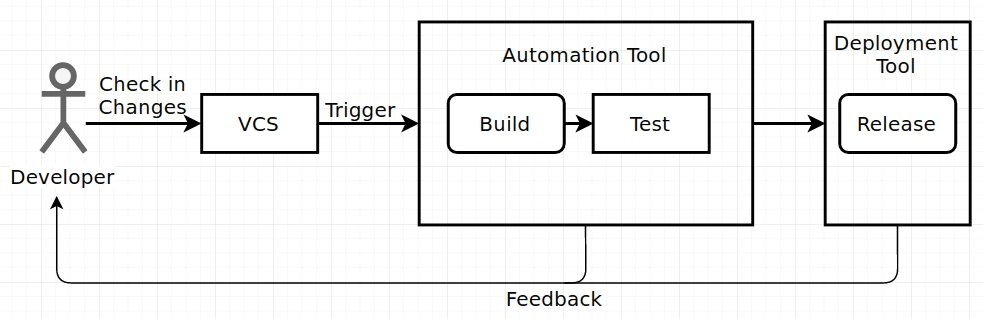
\includegraphics[scale=0.45]{images/pipeline-simple.jpg}
	\caption{The pipeline made simple}
	\label{fig:pipeline-simple}
\end{figure}

The developer will check in the code to the VCS witch in turn will trigger the automation tool. The automation tool will then build the project and test, before sending it out to release. If any of the stages fail the rest of the pipeline is not ran and feedback is sent to the developer so they can fix it.
\\\\
The testing part of the pipeline refers to unit tests and the other forms mentioned in the earlier chapters. Even on a full pass the feedback will be sent, this will help guard against false positives.
\\\\
When talking about the architecture such a system there are two side, firstly the software pipeline as seen above. How each of the steps flow into each over and what is needed to pass between each of the steps. The second is the hardware layout,  such as are the unit tests ran of the same server that it is built, or maybe the entire pipeline in confined to a single server.

\subsection{Software architecture}

Figure \ref{fig:pipeline-simple} showed a basic pipeline for a continuous delivery pipeline, however there is not enough details to build a system from this. Below figure \ref{fig:bsipipeline} shows the system developed from the project that sparked this paper:

\begin{figure}[H]
	\centering
	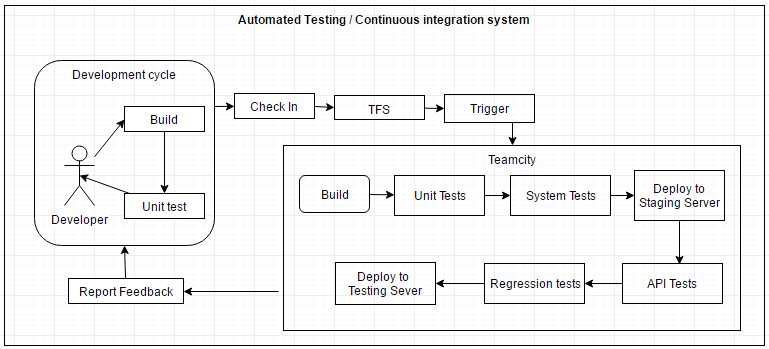
\includegraphics[scale=0.6]{images/bsipipleine.png}
	\caption{A full delivery pipeline}
	\label{fig:bsipipeline}
\end{figure}

The figure shows two things, firstly it reveals the local development cycle. The cycle being that the developer will check the basics before checking in the code to the VCS in this case a TFS server. Not noted on the diagram the developer will also have access to a local running copy of the program allowing them to run other forms of tests if needed. 
\\\\
The second part, it expands on the build and test block previously seen, firstly, the build, then the unit tests followed by system tests. System not mention before are tests a form of integration tests. This then leads on to a interesting part where the system is deployed on a staging instance, this allows the API and regression tests to be ran, as they require a the full system up and running. This is then deployed to testing  for manual tests, where it can then be pushed to production.
\\\\
The interesting part here is how four different deployments are needed, one for the developer, one for staging, one for testing and one for production. This is where Docker and other such tools fit into the picture.
\\\\
This kind of pipeline is a common one, some may use different types of tests as it will suite their needs better, but the theme is still the same. One such system by \cite{zend} adds an additional step after build to package the system up, ready to deploy, and as mentioned they have swapped out the test types for that which suit their product.
\\\\
Another interesting take on this by \cite{codeahoy}, has split their project into different components, this means rather than having one project to handle integration tests, both system to to be build and then integrated together. Therefore they used the architecture in figure \ref{fig:codeahoy}:

\begin{figure}[H]
	\centering
	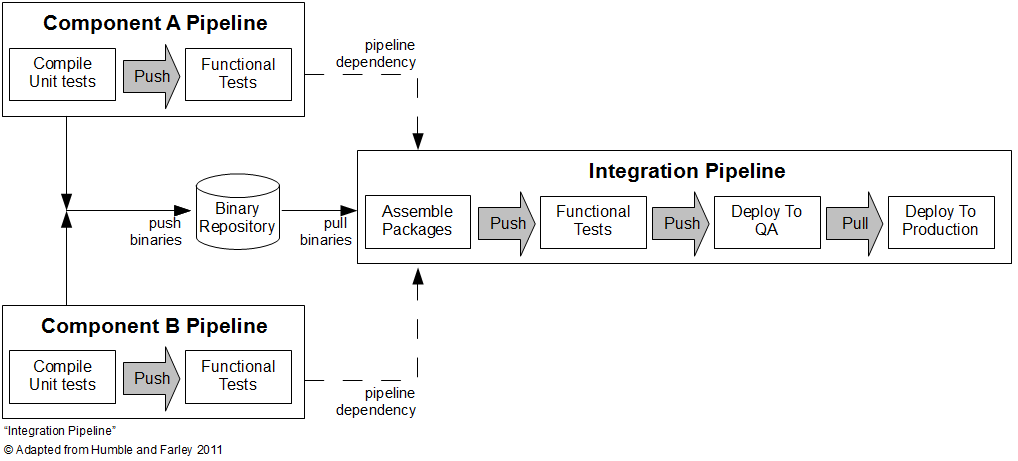
\includegraphics[scale=0.5]{images/codeahoy.png}
	\caption{A dual channel delivery pipeline by \cite{codeahoy}}
	\label{fig:codeahoy}
\end{figure}

This design has added an additional repository for binaries, then when a commit is placed in component A or B, it can progress through the entire pipeline by getting the latest version of the other components binaries from the repository. 
\\\\
\cite{thoughworks} takes this a step further by not only splitting the pipeline into separate components  but also places them in different repositories, making the first time they are integrated together being the integration tests as they all come from their own binary repositories.
\\\\
This kind of pattern goes along with the development environments based on breaking up a monolith architecture of a project into smaller more manageable units. This system makes it easy to add continuous deployment into micro service an other types of modular architecture.
\\\\
One thing not show so far but some teams find invaluable is to run a static analysis on the code base to pre-emptively spot erroneous areas in the project before they happen. This can then be sent back with the rest of the report to the developers and other interested parties.
\\\\
This basic pattern and flow of the pipeline does seems to be a common theme throughout all over implementations.  With the single monolith structure taking it from the start to end and the second combining multiple components into a single software package. 

\subsection{VCS workflow}

As seen the pipeline is generally triggered via a commit into the VCS this makes the workflow with the branch structure and VCS a central component into how the rest of the systems are put together.
\\\\
There are two main schools of thoughts when working with continuous deployment and VCS the first is more commonly seen in open source projects that are hosted on sites such as Github and Bitbucket, with the second when everyone has full access to the repository. 
\\\\
The fist uses a pull request system, all the developers or contributes to the project will submit their changes trough a pull request. When the request is made an automated system will start the process of running through the pipeline. 
\\\\
Here the system can automatically merge the change if it passes, however, in open source project it is more common to find the owners to perform a code review and check for harmful changes before merging the request manually. If however it is a private repository the code checked in can be automatically merged. 
\\\\
If the checks fail the request can remain open util an update is pushed to it where it will run the checks again. This is visualised in figure \ref{fig:osspipeline}.

\begin{figure}[H]
	\centering
	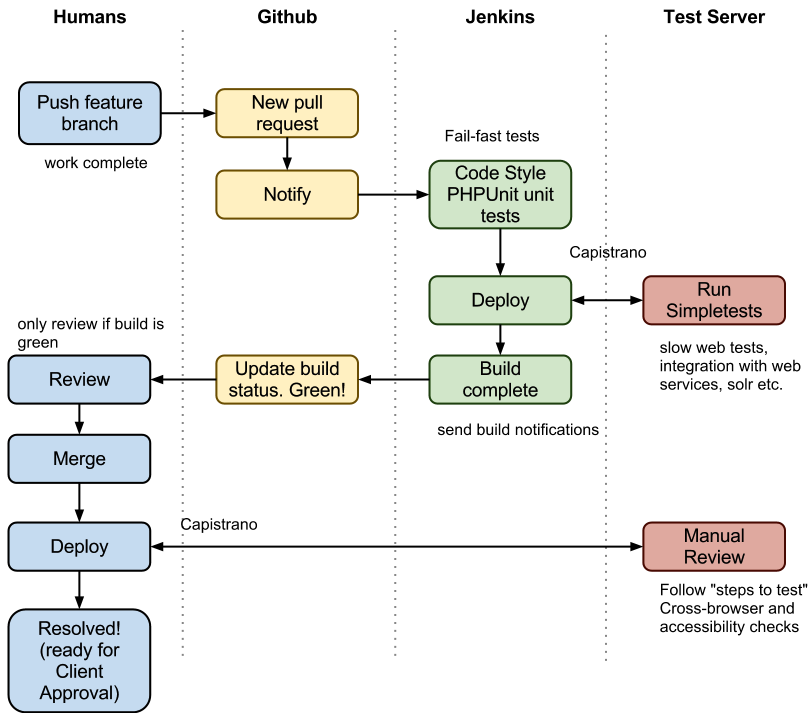
\includegraphics[scale=0.4]{images/osspipeline.png}
	\caption{Pull request delivery pipeline by \cite{osspipeline}}
	\label{fig:osspipeline}
\end{figure}

The only thing to note about the diagram is the manual review as mentioned, this could be automated creating the full continuous delivery pipeline rather than continuous integration.
\\\\
The second system is similar to the pull request however rather than preforming the change in a pull request the commit is placed inside the teams VCS workflow branch. When working in a agile and continuous delivery environment it is general accepted that there should be a master branch that is the latest version of the software. This is also the branch where all the development goes and what the customer gets.
\\\\
Following that system the main branch will have the pipeline attached, when a milestone is reached such as the end of a sprint in agile methodology. A new branch is created to represent the milestone at that point in time. 
\\\\
One reason for this workflow is it will carry well across multiple systems as TFS does not branch in the same way that GIT does. Branching in GIT is similar to changing the entire repository, for example if the current branch is master, then when changing to feature\_one branch it is like renaming the folder and swapping its contents. Think of it like a magic room that changes depending on what branch its on. TFS on the other hand is located on a different path, so rather than a single magic room, its will create a new room for each branch.
\\\\
This difference in design will affect how the automation tool will interact with the VCS, as if it is developed using GIT, the system can watch multiple branches at the same time as it is all located in the same place. Whereas with TFS a new configuration will have to be made for each branch as they are separate from each other.
\\\\
With this in mind, if the workflow used is to create a new branch per version work on it until release then repeat, at the end of every release a new configuration will have to be made for the new branch. While this does not vary from the other workflow in terms of branching, new configuration will not have to be made as they will also be branched off with the project as seen in the next part. But, as development is performed on a single branch there is nothing to change until the project does.
\\\\
Before delving into the why the a new configuration is not needed, the master branch of the project as defied must always be in working condition ready to be delivered the users. If commit are therefore placed directly in master and they make the build or tests fail, then the entire concept of continuous deployment is failed as master is not in a  production ready state.
\\\\
In order to combat this the preferred workflow is to use a feature branches, similar to that of a pull request system, development is performed on another branch then when ready can be merged into the master. Similar this allows tests and other action to be perform on the changes fore they are merged into master. This assures that the master will be kept in a working condition.
\\\\
This will also allow the merge to be reverted if there is an issue in the integration without losing the work performed as more commit can be made and tried to merge again.
\\\\
Now that there is a workflow in place and the pipeline is ready to be attached to the branches, where does the code and other parts needed in the pipeline go. The tools such as Jenkins, Teamcity and cruisecontrol all offer the ability to store scripts inside their systems through their user interface.
\\\\
For example Teamcity comes with pre-scripted runners that will allow a click and select experience to get the entire system set-up. While this is certainly a good selling point for non-experienced or quick one time set-ups over the long term this could be quite the opposite. In multiple ways, if the team decides they want to change from Teamcity to Jenkins now the entire system has to be built from the ground up again. Otherwise it might end up try to fit the way Teamcity handles things into Jenkins.
\\\\
Other issues with software version setting up new branches and so on, there are many more reasons as to why it is good in the short term on small project but for larger and more longer terms a better system is needed.
\\\\
Rather than storing the scripts inside of the tool, they should be placed inside of the VCS then depending on the set up, just have to call a single or multiple external scripts from the tool even if the scripts are a single line. In an ideal situation the scripts should be able to run on the target platforms for the project, such as using python or ruby rather than bash and batch file, to save writing them twice.
\\\\
This also has the befits of someone to walk up to a brand new machine get the repository and have the full system up and running within minutes as the VCS holds all the scripts needed.

\subsection{Hardware architecture}

Up to this point the paper has focused on the software side of thing looking at the pipeline, VCS and scripts. This next section will look at where this is hosted and how where each part can be split.  



\subsection{Architecture final thoughts}
